\documentclass{bmstu}

\bibliography{biblio}

\begin{document}

\makereporttitle
    {Информатика и системы управления}
    {Программное обеспечение ЭВМ и информационные технологии}
    {лабораторной работе №~2}
    {Анализ алгоритмов}
    {}
    {}
    {Новиков~А.~А./ИУ7-52Б}
    {Строганов~Д.~В.}

\renewcommand{\contentsname}{СОДЕРЖАНИЕ} 
\tableofcontents
\setcounter{page}{2}

\begin{center}
    \textbf{ВВЕДЕНИЕ}
\end{center}
\addcontentsline{toc}{chapter}{ВВЕДЕНИЕ}

Поиск заданного значения в массиве или проверка существования этого значения в нем --- часто встречающаяся задача при работе с массивами. Существуют различные алгоритмы для поиска заданного значения.

\textbf{Цель лабораторной работы} --- исследование алгоритмов умножения матриц следующими методами:
\begin{itemize}
    \item[---] классическим методом;
    \item[---] алгоритм Винограда;
    \item[---] оптимизированного алгоритма Винограда.
\end{itemize}

Для достижения поставленной цели необходимо выполнить следующие задачи:
\begin{itemize}
    \item[---] разобрать указанные алгоритмы умножения матриц;
    \item[---] выполнить оценку трудоемкости алгоритмов;
    \item[---] реализовать алгоритмы умножения матриц: классический, алгоритм Винограда, оптимизированный алгоритм Винограда;
    \item[---] выполнить замеры используемого процессорного времени алгоритмами в зависимости от размера входных матриц;
    \item[---] описать полученные результаты в отчете.
\end{itemize}
\chapter{Аналитический раздел}

В данном разделе будет сформулирована задача коммивояжера, а также будут рассмотрены 2 метода решения этой задачи: муравьиный алгоритм и алгоритм
полного перебора.

\section{Формулировка задачи коммивояжера}

Пусть задан граф $G = (V, E)$, где $V$ --- множество вершин ($|V|=n$), а $E$ --- множество рeбер ($|E|=m$). Каждое ребро ($(i,j)\in E$ имеет длину $c_{ij}$, определяемую матрицей расстояний $C=||c_{ij}||$. Если между вершинами $i$ и $j$ отсутствует ребро, соответствующий элемент матрицы принимается равным бесконечности ($c_{ij} = \infty$)~\cite{com_info}.

Подмножество попарно несмежных ребер графа $G$ называется паросочетанием. Паросочетание считается совершенным, если каждая вершина графа инцидентна ровно одному ребру из этого множества. Совокупность простых попарно непересекающихся циклов, покрывающая все вершины графа $G$, называется 2-фактором. Если 2-фактор состоит из одного цикла, то он называется гамильтоновым циклом~\cite{gamelton}.

Задача заключается в поиске гамильтонова цикла минимальной длины, то есть цикла, который проходит через каждую вершину графа ровно один раз и возвращается в начальную точку.


\subsection{Алгоритм полного перебора}
Алгоритм полного перебора для решения задачи коммивояжера основывается на проверке всех возможных маршрутов в графе для определения минимального. Этот метод заключается в полном переборе всех вариантов обхода городов и выборе маршрута с наименьшей длиной. Однако количество возможных маршрутов быстро растет с увеличением числа городов $n$, поскольку сложность алгоритма составляет $n!$. Несмотря на то, что данный подход гарантирует получение точного решения, его применение становится крайне неэффективным даже при относительно небольшом количестве городов из-за значительных вычислительных затрат.

\subsection{Муравьиный алгоритм}
В основе муравьиного алгоритма лежит идея моделирования поведения колонии муравьев. Каждый муравей определяет свой маршрут на основе оставленных другими муравьями феромонов, а также сам оставляет оставляет феромоны, чтобы последующие муравьи ориентировались по ним. В результате при прохождении каждым муравьем своего маршрута наибольшее число феромонов остается на самом оптимальном пути. Временная сложность алгоритма была оценена как $683 - (42,467 · N) + (1,0696 · N^2)$~\cite{ants}. Однако главный недостаток алгоритма заключается в том, что, по сравнению с алгоритмом полного перебора, он дает приближенное решение задачи, а не точное.

Вероятность перехода муравья $k$ из текущей вершины $i$ в вершину $j$ рассчитывается по формуле:
\begin{equation}
    \label{posib}
    P_{kij} = 
    \begin{cases}
        \frac{\tau_{ij}^a \eta_{ij}^b}{\sum_{q \in J_{ik}} \tau_{iq}^a \eta_{iq}^b}, & \text{если вершина $j$ еще не посещена муравьем $k$,} \\
        0, & \text{иначе,}
    \end{cases}
\end{equation}
где:
\begin{itemize}
    \item[---] $a$ --- параметр влияния феромона;
    \item[---] $b$ --- параметр влияния длины пути;
    \item[---] $\tau_{ij}$ --- количество феромонов на ребре $(i, j)$;
    \item[---] $\eta_{ij}$ --- видимость (величина обратная расстоянию до вершины).
\end{itemize}

По окончанию движения всех муравьев уровень феромонов на ребрах обновляется по формуле:
\begin{equation}
    \label{update_phero_1}
    \tau_{ij}(t+1) = (1-p)\tau_{ij}(t) + \Delta \tau_{ij},
\end{equation}

где $p$ — коэффициент испарения феромона, а $\Delta \tau_{ij}$ определяется как:

\begin{equation}
    \label{update_phero_2}
    \Delta \tau_{ij} = \sum_{k=1}^N \Delta \tau_{ij}^k,
\end{equation}

\begin{equation}
    \label{update_phero_3}
    \Delta \tau_{ij}^k = 
    \begin{cases}
        \frac{Q}{L_k}, & \text{если ребро $(i, j)$ посещено муравьем $k$,} \\
        0, & \text{иначе,}
    \end{cases}
\end{equation}

где $Q$ — параметр, связанный с длиной оптимального пути, а $L_k$ — длина маршрута муравья $k$.

\subsection{Описание алгоритма}
Пошаговое описание муравьиного алгоритма:
\begin{enumerate}
    \item[1)] Муравей исключает из дальнейшего выбора вершины, которые уже были посещены, ссылаясь на список посещенных вершин, хранящийся в его памяти (список запретов $J_{ik}$).
    \item[2)] Муравей оценивает привлекательность вершин, основываясь на их видимости, которая обратно пропорциональна расстоянию между ними.
    \item[3)] Муравей ощущает уровень феромонов на ребрах графа, что помогает ему определять предпочтительность маршрута.
    \item[4)] После прохождения ребра $(i, j)$ муравей оставляет на нем феромоны, количество которых зависит от длины маршрута $L_k$, пройденного муравьем, и параметра $Q$.
\end{enumerate}

\textbf{ВЫВОД}

В данном разделе была представлена формулировка задача коммивояжера, а также рассмотрены 2 метода ее решения: муравьиный алгоритм и алгоритм полного перебора

\chapter{Конструкторский раздел}
В данном разделе будут определены требования к программному обеспечению
и приведены схемы алгоритма полного перебора и муравьиного алгоритма для
решения задачи коммивояжера.

\section{Требования к программному обеспечению}
Входные данные: матрица стоимостей взвешенного неориентированного графа.

Выходные данные: кратчайший гамильтонов цикл.

\section{Представления алгоритмов}
На рисунках~\ref{fig:brute_force}~---~\ref{fig:ant} представлены схема алгоритма полного перебора и схема муравьиного алгоритма.

\begin{figure}[H]
    \centering
    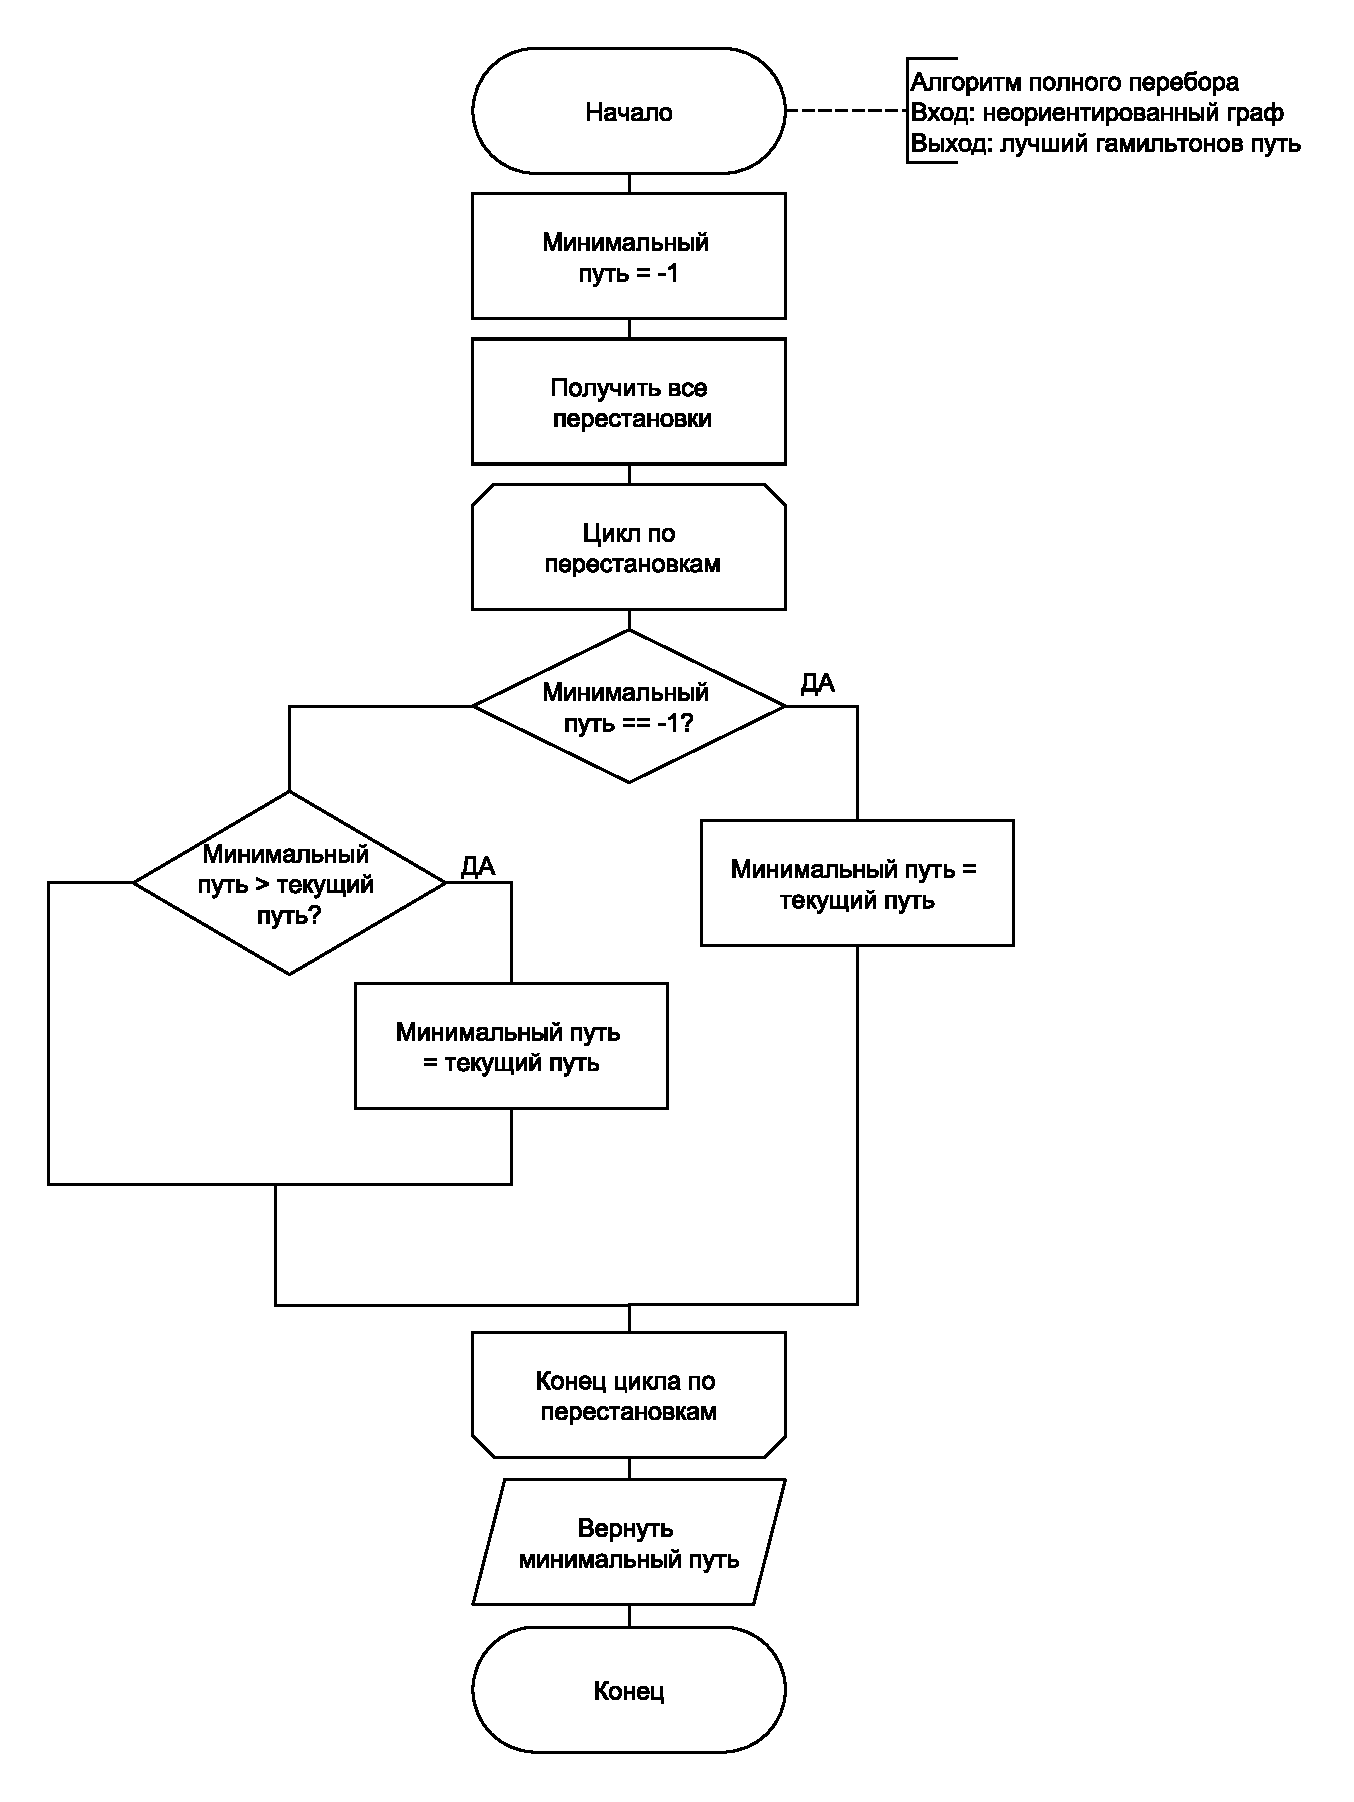
\includegraphics[scale=0.7]{img/unnamed1.eps}
    \caption{Схема алгоритма полного перебора}
    \label{fig:brute_force}
\end{figure}

\begin{figure}[H]
    \centering
    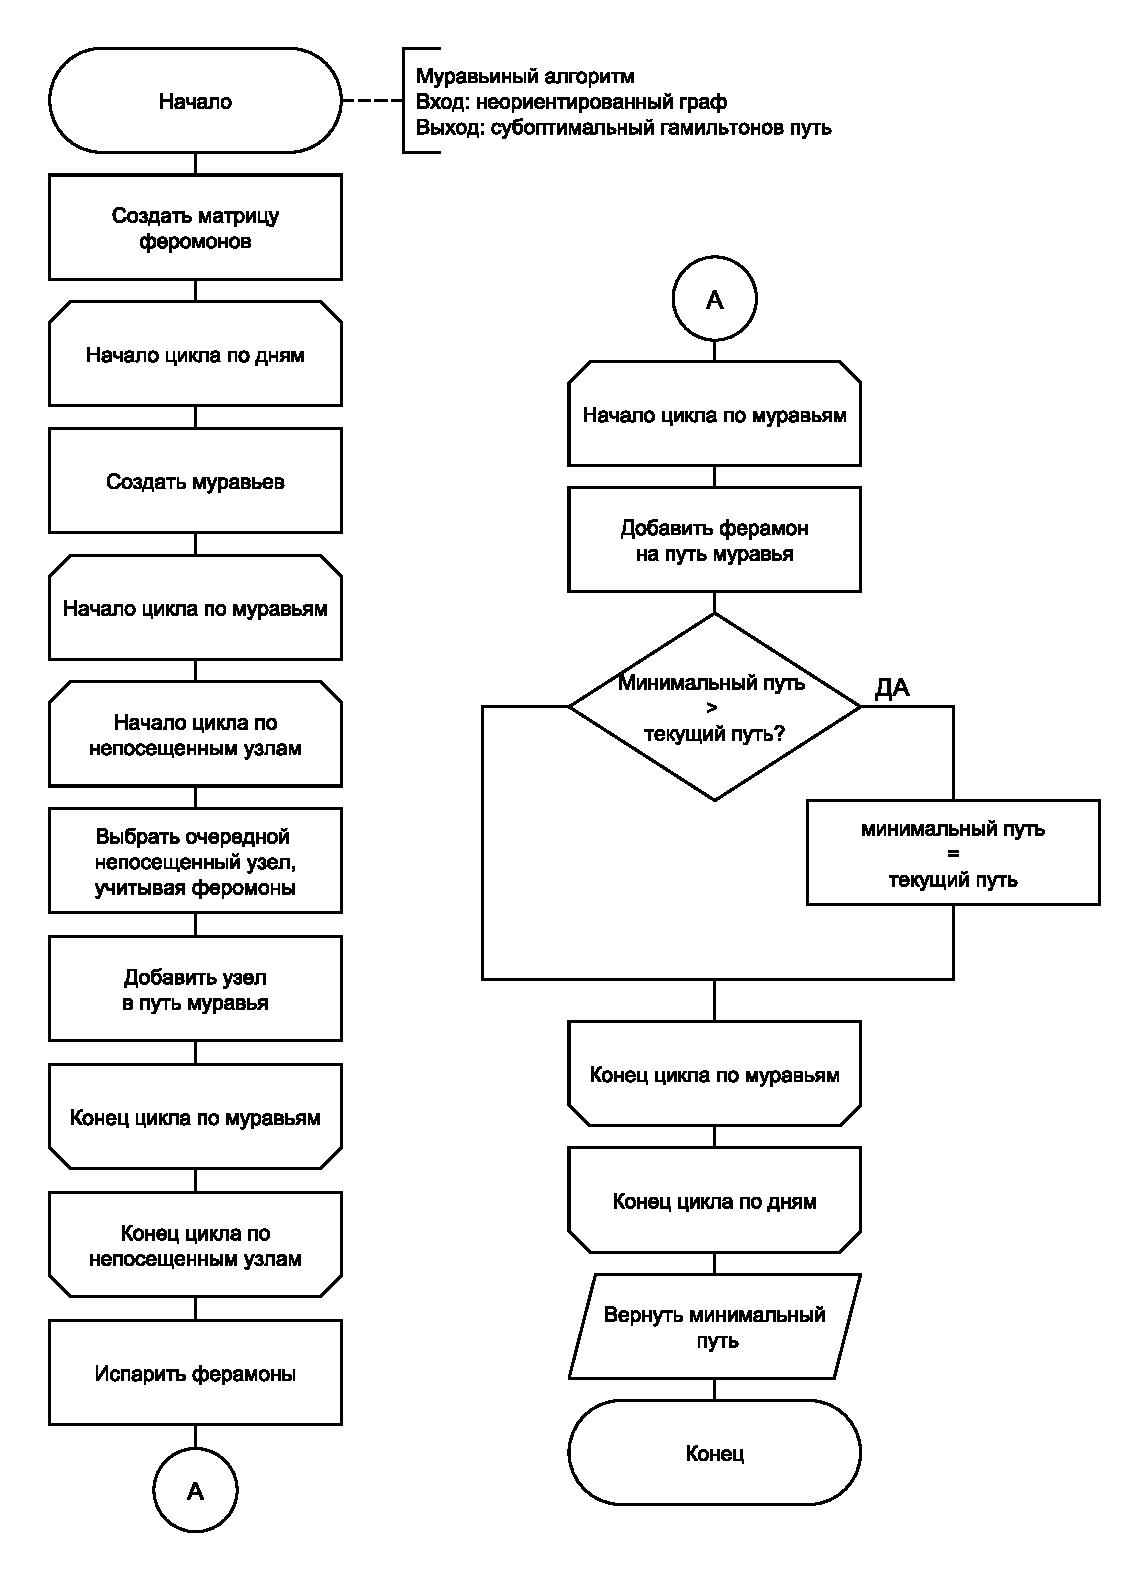
\includegraphics[scale=0.7]{img/unnamed2.eps}
    \caption{Схема муравьиного алгоритма}
    \label{fig:ant}
\end{figure}

\textbf{ВЫВОД}

В данном разделе были определены требования к программному обеспечению и приведены схемы алгоритмов полного перебора и муравьиного алгоритма для решения задачи коммивояжера.

\clearpage
\chapter{Технологический раздел}

В данном разделе описаны требования к программному обеспечению, реализация алгоритмов и средства реализации.

\section{Требования к программному обеспечению}

Входные данные: две матрицы, количество столбцов первой матрицы равно количеству строк второй матрицы;
Выходные данные: матрицы, являющаяся произведением вхожных матриц.


\section{Средства реализации}
Для реализации данной лабораторной работы выбран язык программирования $C$ \cite{C}. Выбор был обусловлен необходимостью производить замеры на микроконтроллерах и наличием библиотеки $time$\cite{C_date}. Время было замерено с помощью функции $clock$\cite{C_clock}.

\section{Реализация алгоритмов}
В листингах \ref{lst:default} --- \ref{lst:vinograd_mod} представлены реализации алгоритмов.

\begin{center}
\captionsetup{justification=raggedright,singlelinecheck=off}
\begin{lstlisting}[language=C, frame=single, numbers=left, label=lst:default, caption=Реализация классического алгоритма]
error_t matrix_mul(const matrix_t *matrix_1, const matrix_t *matrix_2, matrix_t *result) {
    if (matrix_1->collumn != matrix_2->row) return ERR_RANGE;
    error_t rc = alloc_matrix_t(result, matrix_1->row, matrix_2->collumn);
    if (rc) return rc;
    for (size_t i = 0; i < result->row; ++i)
    {
        for (size_t j = 0; j != result->collumn; ++j)
        {
            result->data[i][j] = 0;
            for (size_t k = 0; k < matrix_1->collumn; ++k)
                result->data[i][j] = result->data[i][j] + matrix_1->data[i][k] * matrix_2->data[k][j];
        }
    }
    return ERR_OK;
}\end{lstlisting}
\end{center}

\clearpage

\begin{center}
\captionsetup{justification=raggedright,singlelinecheck=off}
\begin{lstlisting}[language=C, frame=single, numbers=left, label=lst:vinograd,caption=Реализация алгоритма Винограда]
error_t vinograd_matrix_mul(const matrix_t *matrix_1, const matrix_t *matrix_2, matrix_t *result) {
    if (matrix_1->collumn != matrix_2->row)
        return ERR_RANGE;

    error_t rc = alloc_matrix_t(result, matrix_1->row, matrix_2->collumn);
    if (rc)
        return rc;

    size_t row_1 = matrix_1->row;
    size_t collumn_1 = matrix_1->collumn;
    size_t collumn_2 = matrix_2->collumn;

    int *row_factor = malloc(row_1 * sizeof(int));
    int *col_factor;
    if (row_factor != NULL) {
        col_factor = malloc(collumn_2 * sizeof(int));
        if (col_factor == NULL) {
            free(row_factor);
            return ERR_MEM;
        }
    } else
        return ERR_MEM;

    for (size_t i = 0; i < row_1; ++i) {
        row_factor[i] = 0;
        for (size_t j = 0; j < collumn_1 / 2; ++j) {
            row_factor[i] = row_factor[i] +
                            matrix_1->data[i][2 * j] * 
                            matrix_1->data[i][2 * j + 1];
        }
    }

    for (size_t j = 0; j < collumn_2; ++j) {
        col_factor[j] = 0;
        for (size_t i = 0; i < collumn_1 / 2; ++i) {
            col_factor[j] = col_factor[j] +
                            matrix_2->data[2 * i][j] * 
                            matrix_2->data[2 * i + 1][j];
        }
    }

    for (size_t i = 0; i < row_1; ++i) {
        for (size_t j = 0; j < collumn_2; ++j) {
            result->data[i][j] = -row_factor[i] - col_factor[j];
            for (size_t k = 0; k < collumn_1 / 2; ++k) {
                result->data[i][j] = result->data[i][j] + 
                (matrix_1->data[i][2 * k] +
                matrix_2->data[2 * k + 1][j]) * 
                (matrix_1->data[i][2 * k + 1] + 
                matrix_2->data[2 * k][j]);
            }
        }
    }

    if (collumn_1 % 2 == 1) {
        for (size_t i = 0; i < row_1; ++i) {
            for (size_t j = 0; j < collumn_2; ++j) {
                result->data[i][j] = result->data[i][j] +
                matrix_1->data[i][collumn_1 - 1] * 
                matrix_2->data[collumn_1 - 1][j];
            }
        }
    }

    free(col_factor);
    free(row_factor);

    return ERR_OK;
}
\end{lstlisting}
\end{center}

\clearpage

\begin{center}
\captionsetup{justification=raggedright,singlelinecheck=off}
\begin{lstlisting}[language=C, frame=single, numbers=left, label=lst:vinograd_mod, caption=Реализация оптимизированного алгоритма Винограда]
error_t vinograd_modify_matrix_mul(const matrix_t *matrix_1, const matrix_t *matrix_2, matrix_t *result) {
    if (matrix_1->collumn != matrix_2->row)
        return ERR_RANGE;

    error_t rc = alloc_matrix_t(result, matrix_1->row, matrix_2->collumn);
    if (rc)
        return rc;

    size_t row_1 = matrix_1->row;
    size_t collumn_1 = matrix_1->collumn;
    size_t collumn_2 = matrix_2->collumn;

    int *row_factor = malloc(row_1 * sizeof(int));
    int *col_factor;
    if (row_factor != NULL) {
        col_factor = malloc(collumn_2 * sizeof(int));
        if (col_factor == NULL) {
            free(row_factor);
            return ERR_MEM;
        }
    } else
        return ERR_MEM;

    for (size_t i = 0; i < row_1; ++i) {
        row_factor[i] = 0;
        for (size_t j = 0; j < collumn_1 / 2; ++j) {
            row_factor[i] += matrix_1->data[i][j << 1] * matrix_1->data[i][(j << 1) + 1];
        }
    }

    for (size_t j = 0; j < collumn_2; ++j) {
        col_factor[j] = 0;
        for (size_t i = 0; i < collumn_1 / 2; ++i) {
            col_factor[j] += matrix_2->data[i << 1][j] * matrix_2->data[(i << 1) + 1][j];
        }
    }

    for (size_t i = 0; i < row_1; ++i) {
        for (size_t j = 0; j < collumn_2; ++j) {
            result->data[i][j] = -row_factor[i] - col_factor[j] +
                                 (matrix_1->data[i][0] + 
                                 matrix_2->data[1][j]) * 
                                 (matrix_1->data[i][1] + 
                                 matrix_2->data[0][j]);
            for (size_t k = 1; k < collumn_1 / 2; ++k) {
                result->data[i][j] += 
                (matrix_1->data[i][k << 1] + 
                matrix_2->data[(k << 1) + 1][j]) *
                (matrix_1->data[i][(k << 1) + 1] + 
                matrix_2->data[k << 1][j]);
            }
        }
    }

    if (collumn_1 % 2 == 1) {
        for (size_t i = 0; i < row_1; ++i) {
            for (size_t j = 0; j < collumn_2; ++j) {
                result->data[i][j] += 
                matrix_1->data[i][collumn_1 - 1] * 
                matrix_2->data[collumn_1 - 1][j];
            }
        }
    }

    free(col_factor);
    free(row_factor);

    return ERR_OK;
}
\end{lstlisting}
\end{center}

\clearpage

\textbf{ВЫВОД}

В данном разделе были представлены реализации алгоритмов умножения матриц, были рассмотрены средства реализации, предъявлены требования к программному обеспечению.
\clearpage
\chapter{Исследовательский раздел}
В данном разделе проведен сравнительный анализ алгоритмов по используемому процессорному времени.

\section{Технические характеристики}
Технические характеристики используемого устройства:
\begin{itemize}
    \item[---] операционная система --- Ubuntu Linux x86\_64~\cite{Ubuntu};
    \item[---] память --- 16 Гб;
    \item[---] процессор --- AMD Ryzen 5 5500U (6x2.10 ГГц)~\cite{AMD}.
\end{itemize}


\section{Время выполнения алгоритмов}
Замеры времени проводились на графах с одинаковым количеством вершин. Каждое значение получено путем взятия среднего из 10 измерений. Результаты замеров приведены в таблице~\ref{tbl:time_measurements}.

\begin{table}[h]
	\begin{center}
		\begin{threeparttable}
		\captionsetup{justification=raggedright,singlelinecheck=off}
		\caption{Время работы алгоритмов (в мс)}
		\label{tbl:time_measurements}
		\begin{tabular}{|c|r|r|r|}
			\hline
			Размер матрицы & Полный перебор & Муравьиный алгоритм \\
            \hline
			1    & 0.115 & 0.863 \\
            \hline
			2    & 0.159 & 0.943 \\ 
            \hline
			3    & 0.081 & 0.948 \\ 
            \hline
			4    & 0.071 & 1.472 \\ 
			\hline
			5    & 0.952 & 2.460 \\ 
			\hline
			6    & 8.413 & 3.565 \\ 
			\hline
			7    & 85.019 & 4.527 \\ 
			\hline
			8    & 862.511 & 5.422 \\ 
			\hline
			9    & 11282.250 & 6.619 \\ 
            \hline
		\end{tabular}
		\end{threeparttable}
    \end{center}
\end{table}

\clearpage

Зависимости времени решения задачи коммивояжера от количества вершин графа для двух алгоритмов представлены на рисунке~\ref{fig:tm}.
\begin{figure}[H]
    \centering
    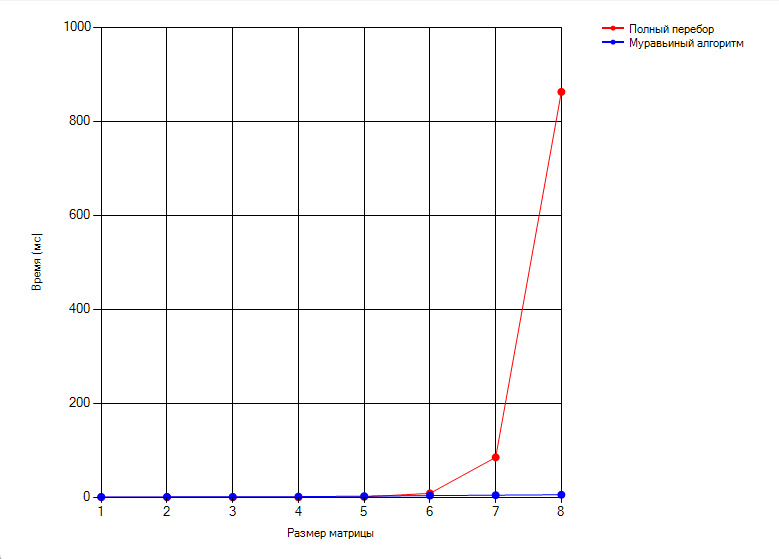
\includegraphics[width=1\linewidth]{img/graph-1.png}
    \caption{Зависимость времени выполнения программы от количества вершин}
    \label{fig:tm}
\end{figure}


\section{Классы данных}
В качестве класс данных для параметризации используются графы, построенные на городах Африке, при этом используется всего 3 графа. В качестве весов использовались расстояния между этими городами по прямой в км~\cite{maps}.

\section{Результаты параметризации}
В результате параметризации оказалось, что самыми лучшими параметрами по заданному классу данных оказались при $\alpha$ = 0.1, $\rho$ = 0.5 и количеством дней равным 50. При этом данные параметры дают лучший результат на всех классах данных и по всем параметрам сравнения. Результаты параметризации для лучших параметров представлены в таблице~\ref{tbl:param}, а
вся таблица параметризации и класс данных представлены в приложении А.


\begin{longtable}{|>{\centering\arraybackslash}r| >{\centering\arraybackslash}r| >{\centering\arraybackslash}r| >{\centering\arraybackslash}r| >{\centering\arraybackslash}r| >{\centering\arraybackslash}r| >{\centering\arraybackslash}r| >{\centering\arraybackslash}r| >{\centering\arraybackslash}r| >{\centering\arraybackslash}r| >{\centering\arraybackslash}r| >{\centering\arraybackslash}r|}
\caption{Результаты параметризации муравьиного алгоритма}\label{tbl:param}
\\ \hline
\multicolumn{3}{|c|}{Параметры} & \multicolumn{3}{|c|}{Граф 1} & \multicolumn{3}{|c|}{Граф 2} & \multicolumn{3}{|c|}{Граф 3} \\
\hline
$\alpha$ & $\rho$ & \text{Дни} & \text{min} & \text{max} & \text{avg} & \text{min} & \text{max} & \text{avg} & \text{min} & \text{max} & \text{avg} \\
\hline
\endfirsthead
\multicolumn{12}{c}{\text{Продолжение на следующей странице}} \\
\hline
\endhead
\hline
\multicolumn{12}{r}{\text{Конец таблицы}} \\
\hline
\endfoot
\endlastfoot
\hline
0.1 & 0.25 & 100 & 0 & 0 & 0 & 0 & 0 & 0 & 0 & 0 & 0 \\ 
0.1 & 0.25 & 200 & 0 & 0 & 0 & 0 & 0 & 0 & 0 & 0 & 0 \\ 
0.1 & 0.5 & 50 & 0 & 0 & 0 & 0 & 0 & 0 & 0 & 0 & 0 \\ 
0.1 & 0.5 & 100 & 0 & 0 & 0 & 0 & 0 & 0 & 0 & 0 & 0 \\ 
0.1 & 0.75 & 200 & 0 & 0 & 0 & 0 & 0 & 0 & 0 & 0 & 0 \\ 
0.25 & 0.1 & 100 & 0 & 0 & 0 & 0 & 0 & 0 & 0 & 0 & 0 \\ 
0.25 & 0.1 & 100 & 0 & 0 & 0 & 0 & 0 & 0 & 0 & 0 & 0 \\ 
0.5 & 0.1 & 200 & 0 & 0 & 0 & 0 & 0 & 0 & 0 & 0 & 0 \\ 
\hline
\end{longtable}


\textbf{ВЫВОД}

В результате исследования было получено, что на графе с вершинами меньше 7 муравьиный алгоритм и алгоритм полного перебора выполняют задачу за примерно одинаковое время, а при количестве вершин большем или равном 7 муравьиный алгоритм работает около в раз быстрее, чем алгоритм полного перебора.

Также было выявлено, что при $\alpha = 0.1$, $\rho = 0.5$ и количеством дней равным 50 муравьиный алгоритм дает наилучшие результаты.
\begin{center}
    \textbf{ЗАКЛЮЧЕНИЕ}
\end{center}
\addcontentsline{toc}{chapter}{ЗАКЛЮЧЕНИЕ}

В процессе работы были исследованы временные и алгоритмические сложности муравьиного алгоритма и метода полного перебора. Также были проведены замеры времени выполнения и параметризация муравьиного алгоритма, что дало возможность определить оптимальные параметры для набора данных, представленного в приложении А. Наилучшие параметры были установлены на уровне:  $\alpha = 0.1$, $\rho=0.5$ и количество дней равным 50.


В ходе выполнения данной лабораторной работы были решены следующие задачи:
\begin{itemize} 
    \item[---] сформулирована задача коммивояжера; 
    \item[---] рассмотреть алгоритмы решения: полным перебором, с использованием муравьиного алгоритма; 
    \item[---] реализовать данные алгоритмы; 
    \item[---] провести сравнительный анализ времени работы алгоритмов; 
    \item[---] выполнить параметризацию для муравьиного алгоритма. 
\end{itemize}
\makebibliography



\end{document}